\chapter{滤波器与传递函数}\label{ch:b1:filters-transfer-functions}

在音箱内部，一个线圈与一个电容器不用任何晶体管，
就决定低音送往大纸盆、高音送往小球顶。
示波器上的“AC”按钮能去掉缓慢漂移的直流偏移，
只保留叠加其上的起伏。电源借助一个电容器，
把脉动的整流市电变为平稳的\omterm{def:b1:dc-circuits:voltage}{电压}。
这三者都是\emph{\omterm{def:b1:filters-transfer-functions:H}{滤波器}}：\omterm{def:b1:dc-circuits:linear}{线性电路}，各自对不同频率
区别对待。任何周期\omterm{def:b1:wave-propagation:signal}{信号}都是正弦波之和，因此知道
电路对每个正弦波的作用——即其\omterm{def:b1:filters-transfer-functions:H}{传递函数}——就等于
知道它对一切\omterm{def:b1:wave-propagation:signal}{信号}的作用。本章定义\omterm{def:b1:filters-transfer-functions:H}{传递函数}，
画出前几章中一阶与二阶电路的\omterm{def:b1:filters-transfer-functions:bode}{伯德图}，
并借此
预测方波经\omterm{def:b1:filters-transfer-functions:H}{滤波器}后的输出形式。

\section{传递函数与伯德图}

\begin{definition}[传递函数]\label{def:b1:filters-transfer-functions:H}
\index{传递函数}\index{增益}\index{滤波器}
\omterm{def:b1:dc-circuits:linear}{线性电路}的输入\omterm{def:b1:dc-circuits:voltage}{电压}为 $\underline U_e$，输出\omterm{def:b1:dc-circuits:voltage}{电压}为
$\underline U_s$（输出端不接任何负载），其
\emph{传递函数}为
\[
\underline H(j\omega) = \frac{\underline U_s}{\underline U_e},
\qquad G(\omega) = \abs{\underline H}, \qquad \varphi(\omega) = \arg\underline H,
\]
其中\emph{增益} $G$（即\omterm{def:b1:wave-propagation:signal}{振幅}之比）与
输出相对于输入的相移 $\varphi$。\emph{滤波器}是指为利用其
频率依赖性而使用的此类电路：\omterm{def:b1:wave-propagation:signal}{振幅}为 $E$ 的正弦量在
$\omega$ 时的输出为 $G(\omega)E\cos(\omega t + \varphi(\omega))$。
\end{definition}

\begin{definition}[分贝；伯德图]\label{def:b1:filters-transfer-functions:bode}
\index{分贝}\index{伯德图}\index{截止频率}\index{通带}
以\emph{分贝}表示的\omterm{def:b1:filters-transfer-functions:H}{增益}为 $G_{\mathrm{dB}} = 20\log_{10}G$：
倍数 $10$ 对应 \qty{20}{dB}，倍数 $2$ 对应 \qty{6}{dB}，$1/\sqrt2$ 对应
\qty{-3}{dB}。\emph{伯德图}以 $G_{\mathrm{dB}}$ 与
$\varphi$ 相对于 $\log_{10}\omega$（或 $f$）作图。\emph{截止
频率}是 $G$ 降至 $G_{\max}/\sqrt2$ 处（较最大值低
\qty{-3}{dB}）；\emph{通带}是指与最大值相差
不超过 \qty{3}{dB} 的频率范围。十倍频程是指频率之比为 $10$，
倍频程是指频率之比为 $2$。
\end{definition}

\begin{method}[滤波器类型的快速判断]\label{met:b1:filters-transfer-functions:nature}
计算之前先看极限情形：频率很低时，电容器
相当于断路，线圈相当于导线；频率很高时情况
恰好相反。把元件替换后，看输出是否等于输入
（通过）还是为零（阻断）。低频通过、高频阻断为低通；
反之为高通；高低频都阻断为带通；高低频都通过为带阻。
再由分压关系计算 $\underline H$。
\end{method}

\section{一阶滤波器}

\begin{proposition}[一阶低通滤波器]\label{prop:b1:filters-transfer-functions:lowpass1}
\index{低通滤波器}\index{积分器}
输出取自 $C$ 两端的 RC 分压电路（或输出取自
$R$ 两端的 RL 分压电路）具有
\[
\underline H = \frac{1}{1 + j\omega/\omega_c}, \qquad
\omega_c = \frac{1}{RC} \ \Big(\text{或 } \frac{R}{L}\Big),
\qquad G = \frac{1}{\sqrt{1 + (\omega/\omega_c)^2}}, \qquad
\varphi = -\arctan\frac{\omega}{\omega_c} .
\]
伯德渐近线：$G_{\mathrm{dB}} = 0$，对应 $\omega \ll \omega_c$；
对 $\omega \gg \omega_c$，直线每十倍频程下降 \qty{20}{dB}，
两线相交于 $\omega_c$，此处精确曲线为 \qty{-3}{dB}，且
$\varphi = -45^\circ$。当 $\omega \gg \omega_c$ 时，$\underline H \approx
\omega_c/(j\omega)$：输出正比于输入的\emph{积分}
——此时\omterm{def:b1:filters-transfer-functions:H}{滤波器}即为积分器。
\end{proposition}

\begin{proof}
分压关系：
\[
\underline H = \frac{1/jC\omega}{R + 1/jC\omega} = \frac{1}{1 + jRC\omega} .
\]
远高于\omterm{def:b1:filters-transfer-functions:bode}{截止频率}时，$1 + j\omega/\omega_c \approx j\omega/\omega_c$，且
将\omterm{def:b1:sinusoidal-impedance:complex}{复振幅}除以 $j\omega$ 即为积分
（见\cref{prop:b1:sinusoidal-impedance:rules}）：$u_s \approx \omega_c\int u_e\,\dd t$。
$20\log(\omega_c/\omega)$ 随 $\omega$ 增大十倍而下降 \qty{20}{dB}。
\end{proof}

\begin{proposition}[一阶高通滤波器]\label{prop:b1:filters-transfer-functions:highpass1}
\index{高通滤波器}\index{微分器}
输出取自 $R$ 两端的 CR 分压电路（或输出取自
$L$ 两端的 LR 分压电路）具有
\[
\underline H = \frac{j\omega/\omega_c}{1 + j\omega/\omega_c},
\qquad G = \frac{\omega/\omega_c}{\sqrt{1 + (\omega/\omega_c)^2}},
\qquad \varphi = \frac{\pi}{2} - \arctan\frac{\omega}{\omega_c},
\]
以 $\omega_c$ 为界，低于它时每十倍频程上升 \qty{20}{dB}，高于它则平坦，
\omterm{def:b1:filters-transfer-functions:H}{增益}为 \qty{-3}{dB}、\omterm{def:b1:wave-propagation:signal}{相位}为 $+45^\circ$，二者均在 $\omega_c$ 处。对于 $\omega \ll \omega_c$，$\underline H
\approx j\omega/\omega_c$：输出正比于
输入的\emph{微分}。
\end{proposition}

\begin{proof}
$\underline H = R/(R + 1/jC\omega) = jRC\omega/(1 + jRC\omega)$;
乘以 $j\omega$ 即为微分。
\end{proof}

\begin{omfigure}
\begin{tikzpicture}
\begin{axis}[omaxis, axis x line=bottom, axis y line=left, xlabel style={at={(axis description cs:0.5,-0.14)}, anchor=north}, width=7.4cm, height=5.2cm, xmode=log, xlabel={$\omega/\omega_c$},
    ylabel={$G_{\mathrm{dB}}$}, xmin=0.01, xmax=100, ymin=-42, ymax=6,
    ytick={0,-20,-40}, yticklabels={$0$,$-20$,$-40$},
    xtick={0.01,0.1,1,10,100}, xticklabels={$10^{-2}$,$10^{-1}$,$1$,$10$,$10^{2}$}]
  \addplot[omExo, dashed, domain=0.01:1, samples=2] {0};
  \addplot[omExo, dotted, domain=0.01:100, samples=2] {-3};
  \addplot[omExo, dashed, domain=1:100, samples=2] {-20*log10(x)};
  \addplot[omDef, thick, domain=0.01:100, samples=200] {-10*log10(1 + x^2)};
  \addplot[omThm, thick, domain=0.01:100, samples=200] {-10*log10(1 + 1/x^2)};
  \node[omDef, font=\footnotesize] at (axis cs:0.05,-7) {低通};
  \node[omThm, font=\footnotesize] at (axis cs:30,-9) {高通};
\end{axis}
\end{tikzpicture}\qquad
\begin{tikzpicture}
\begin{axis}[omaxis, axis x line=bottom, axis y line=left, xlabel style={at={(axis description cs:0.5,-0.14)}, anchor=north}, width=7.0cm, height=5.2cm, xmode=log, xlabel={$\omega/\omega_c$},
    ylabel={$\varphi$}, xmin=0.01, xmax=100, ymin=-1.8, ymax=1.8,
    ytick={-1.5708,-0.7854,0,0.7854,1.5708}, yticklabels={$-\frac{\pi}{2}$,$-\frac{\pi}{4}$,$0$,$\frac{\pi}{4}$,$\frac{\pi}{2}$},
    xtick={0.01,0.1,1,10,100}, xticklabels={$10^{-2}$,$10^{-1}$,$1$,$10$,$10^{2}$}]
  \addplot[omDef, thick, domain=0.01:100, samples=200] {-rad(atan(x))};
  \addplot[omThm, thick, domain=0.01:100, samples=200] {rad(90 - atan(x))};
\end{axis}
\end{tikzpicture}

{\small 一阶低通（蓝色）与高通（红色）的\omterm{def:b1:filters-transfer-functions:bode}{伯德图}：
\omterm{def:b1:filters-transfer-functions:H}{增益}以\omterm{def:b1:filters-transfer-functions:bode}{分贝}表示，渐近线（虚线）相交于
\omterm{def:b1:filters-transfer-functions:bode}{截止频率}处，真实\omterm{def:b1:filters-transfer-functions:H}{增益}为 \qty{-3}{dB}，\omterm{def:b1:wave-propagation:signal}{相位}
在此处穿过 $\mp45^\circ$。}
\end{omfigure}

\begin{example}[交流耦合]\label{ex:b1:filters-transfer-functions:accoupling}
示波器的交流输入是\omterm{def:b1:filters-transfer-functions:bode}{截止频率}为 $f_c \approx \qty{10}{Hz}$ 的\omterm{prop:b1:filters-transfer-functions:highpass1}{高通滤波器}：
叠加在 \qty{5}{V} 直流偏置上的 \qty{1}{kHz} \omterm{def:b1:wave-propagation:signal}{信号}，去掉偏置后
以 \qty{-0.0002}{dB} 通过。但 \qty{50}{Hz} 的方波
会明显失真——其平顶下垂——因为在
\qty{50}{Hz} 时，\omterm{def:b1:filters-transfer-functions:H}{滤波器}仅高出其\omterm{def:b1:filters-transfer-functions:bode}{截止频率}一个十倍频程，而
\omterm{def:b1:wave-propagation:signal}{信号}的低次谐波\omterm{def:b1:wave-propagation:signal}{相位}已发生移动
（见\cref{exo:b1:filters-transfer-functions:12}）。
\end{example}

\section{二阶滤波器}

\begin{proposition}[串联 RLC 作为三种滤波器]\label{prop:b1:filters-transfer-functions:rlc}
\index{带通滤波器}\index{二阶滤波器}
令 $x = \omega/\omega_0$，$\omega_0 = 1/\sqrt{LC}$，$Q =
\sqrt{L/C}/R$，由 $\underline U_e$ 驱动的串联 RLC 电路，
根据输出取在何处，有：
\begin{align*}
\text{跨 } C:&\quad \underline H = \frac{1}{1 - x^2 + jx/Q}, \\
\text{跨 } R:&\quad \underline H = \frac{jx/Q}{1 - x^2 + jx/Q} = \frac{1}{1 + jQ(x - 1/x)}, \\
\text{跨 } L:&\quad \underline H = \frac{-x^2}{1 - x^2 + jx/Q}:
\end{align*}
分别是二阶低通、带通和\omterm{prop:b1:filters-transfer-functions:highpass1}{高通滤波器}。远离
$\omega_0$ 时，低通与高通每十倍频程衰减 \qty{40}{dB}，
带通两侧各以每十倍频程 \qty{20}{dB} 衰减；带通
的最大值 $1$ 位于 $\omega_0$，带宽 $\Delta\omega =
\omega_0/Q$，即\cref{thm:b1:sinusoidal-impedance:resonance}中的带宽。
\end{proposition}

\begin{proof}
由总\omterm{def:b1:sinusoidal-impedance:impedance}{阻抗} $R + j(L\omega - 1/C\omega)$ 构成\omterm{prop:b1:dc-circuits:dividers}{分压器}；
分子分母同乘 $jC\omega$，并利用
$LC\omega_0^2 = 1$，$RC\omega_0 = 1/Q$。带通即前一章的电流
谐振，此处读作 $R$ 两端的\omterm{def:b1:dc-circuits:voltage}{电压}。
\end{proof}

\begin{proposition}[二阶低通：$Q$ 的作用]\label{prop:b1:filters-transfer-functions:lowpass2}
\index{共振!滤波器的}
对于低通，$G = 1/\sqrt{(1 - x^2)^2 + x^2/Q^2}$：
当 $Q > 1/\sqrt2$ 时，\omterm{def:b1:filters-transfer-functions:H}{增益}升至 $1$ 以上，在 $\omega_0$ 附近
出现谐振（峰值 $\approx Q$，$Q$ 较大时）；当 $Q = 1/\sqrt2$ 时为“最大平坦”，
$G = 1/\sqrt{1 + x^4}$，在 $\omega_0$ 处恰为 \qty{-3}{dB}；对于更小的
$Q$，\omterm{def:b1:filters-transfer-functions:H}{增益}较早下降。\omterm{def:b1:wave-propagation:signal}{相位}从 $0$ 变到 $-\pi$，经过 $-\pi/2$
即在 $\omega_0$ 处。
\end{proposition}

\begin{proof}
$(1 - x^2)^2 + x^2/Q^2 = 1 + x^4 + x^2(1/Q^2 - 2)$：中间项
在 $Q^2 = \tfrac12$ 时为零，取更大值时为负（峰），
取更小值时为正（下垂）；$x = 1$ 附近的行为
已在\cref{prop:b1:sinusoidal-impedance:overvoltage}中分析。
\end{proof}

\begin{omfigure}
\begin{tikzpicture}
\begin{axis}[omaxis, axis x line=bottom, axis y line=left, xlabel style={at={(axis description cs:0.5,-0.14)}, anchor=north}, width=7.4cm, height=5.4cm, xmode=log, xlabel={$\omega/\omega_0$},
    ylabel={$G_{\mathrm{dB}}$}, xmin=0.1, xmax=10, ymin=-45, ymax=15,
    ytick={10,0,-20,-40}, xtick={0.1,1,10}, xticklabels={$0.1$,$1$,$10$},
    legend style={at={(0.03,0.03)}, anchor=south west, font=\footnotesize, draw=none, fill=none}]
  \addplot[omDef, thick, domain=0.1:10, samples=300] {-10*log10((1 - x^2)^2 + x^2/9)};
  \addlegendentry{$Q = 3$}
  \addplot[omThm, thick, domain=0.1:10, samples=300] {-10*log10(1 + x^4)};
  \addlegendentry{$Q = 1/\sqrt2$}
  \addplot[omProp, thick, domain=0.1:10, samples=300] {-10*log10((1 - x^2)^2 + x^2/0.04)};
  \addlegendentry{$Q = 0.2$}
  \addplot[omExo, dashed, domain=1:10, samples=2] {-40*log10(x)};
\end{axis}
\end{tikzpicture}\qquad
\begin{tikzpicture}
\begin{axis}[omaxis, axis x line=bottom, axis y line=left, xlabel style={at={(axis description cs:0.5,-0.14)}, anchor=north}, width=7.0cm, height=5.4cm, xmode=log, xlabel={$\omega/\omega_0$},
    ylabel={$G_{\mathrm{dB}}$}, xmin=0.1, xmax=10, ymin=-45, ymax=5,
    ytick={0,-20,-40}, xtick={0.1,1,10}, xticklabels={$0.1$,$1$,$10$},
    legend style={at={(0.03,0.97)}, anchor=north west, font=\footnotesize, draw=none, fill=none}]
  \addplot[omExo, dotted, domain=0.1:10, samples=2, forget plot] {-3};
  \addplot[omDef, thick, domain=0.1:10, samples=400] {-10*log10(1 + 100*(x - 1/x)^2)};
  \addlegendentry{$Q = 10$}
  \addplot[omThm, thick, domain=0.1:10, samples=300] {-10*log10(1 + (x - 1/x)^2)};
  \addlegendentry{$Q = 1$}
\end{axis}
\end{tikzpicture}

{\small \omterm{prop:b1:filters-transfer-functions:rlc}{二阶滤波器}由串联 RLC 得到。左图为低通
（输出取在 $C$ 两端），三种 $Q$：出现谐振峰、最大平坦
响应或较早下降，三者都汇入虚线所示的 \qty{-40}{dB/\text{十倍频程}}
渐近线。右图为带通（输出取在 $R$ 两端）：一个宽度
为 $\omega_0/Q$ 的峰，两侧以 \qty{20}{dB/\text{十倍频程}} 下降。}
\end{omfigure}

\begin{example}[分频器]\label{ex:b1:filters-transfer-functions:crossover}
扬声器的低音单元与高音单元各为 \qty{8}{\ohm}，共用
同一功率放大器，经低通（串联线圈）与高通（串联
电容器）的\omterm{def:b1:filters-transfer-functions:bode}{截止频率}为 \qty{2}{kHz}：$L = R/\omega_c = \qty{0.64}{mH}$，
$C = 1/R\omega_c = \qty{10}{\micro F}$。在 \qty{2}{kHz} 处，每个单元获得
\qty{-3}{dB}，即一半功率，并且对每个频率都有 $G_L^2 + G_H^2 = 1$：
功率被分配，而非损失。周末问题要求设计
一个更陡的版本。
\end{example}

\section{周期信号的滤波}

\begin{theorem}[傅里叶分解]\label{thm:b1:filters-transfer-functions:fourier}
\index{傅里叶级数}\index{谐波}\index{频谱!周期信号的}
周期为 $T = 2\pi/\omega$ 的周期\omterm{def:b1:wave-propagation:signal}{信号}（足够规则）等于
一个常数与频率为 $\omega$ 整数倍的一系列正弦函数之和：
\[
s(t) = c_0 + \sum_{n = 1}^{\infty} c_n\cos(n\omega t + \varphi_n),
\]
其中 $c_0 = \langle s\rangle$ 为其平均值；$n = 1$ 项为
\emph{基波}，其余各项为\emph{谐波}，
\omterm{def:b1:wave-propagation:signal}{振幅} $c_n$ 构成\emph{频谱}。幅值为
$\pm E$ 的方波，$c_n = 4E/(n\pi)$（$n$ 为奇数）、$0$（$n$ 为偶数）；幅值为
$\pm E$ 的三角波，$c_n = 8E/(n\pi)^2$（$n$ 为奇数）。
\end{theorem}
\admitted

\begin{remark}[要点]\label{rem:b1:filters-transfer-functions:fourier}
定理以及 $c_n$ 的计算属于本科二年级的数学课程。
这里它只是一种工具：尖角需要很多
谐波（方波的系数仅按 $1/n$ 衰减），光滑\omterm{def:b1:wave-propagation:signal}{信号}
只需很少的谐波（三角波的系数按 $1/n^2$ 衰减）。\omterm{def:b1:wave-propagation:signal}{信号}的谐波成分
正是乐器音色的构成，也是\omterm{def:b1:filters-transfer-functions:H}{滤波器}作用的对象。
\end{remark}

\begin{proposition}[周期信号的线性滤波]\label{prop:b1:filters-transfer-functions:filtering}
通过\omterm{def:b1:filters-transfer-functions:H}{传递函数}为 $\underline H$ 的\omterm{def:b1:filters-transfer-functions:H}{滤波器}后，定理中的
\omterm{def:b1:wave-propagation:signal}{信号}变为
\[
s_{\text{输出}}(t) = G(0)\,c_0 + \sum_{n \geq 1} G(n\omega)\,c_n\cos\!\big(n\omega t + \varphi_n + \varphi(n\omega)\big):
\]
每个谐波按\emph{其自身}频率处的\omterm{def:b1:filters-transfer-functions:H}{增益}缩放，
并按该频率处的\omterm{def:b1:wave-propagation:signal}{相位}平移，然后将各项相加。由此可得：
\begin{itemize}
  \item 当 $\omega_c \ll \omega$ 时，低通\omterm{def:b1:filters-transfer-functions:H}{滤波器}基本只保留 $c_0$：
        它\emph{求平均}（平滑、去除纹波），并把
        方波变成一个小的三角波（积分）；
  \item 当 $\omega_c \ll \omega$ 时，\omterm{prop:b1:filters-transfer-functions:highpass1}{高通滤波器}去掉 $c_0$，并让
        其余部分通过（交流耦合）；当 $\omega_c \gg \omega$ 时，它
        进行微分（方波边沿处出现尖峰）；
  \item 调谐于 $n\omega$ 且 $Q \gg 1$ 的\omterm{prop:b1:filters-transfer-functions:rlc}{带通滤波器}提取出
        第 $n$ 次谐波本身：从方波中分离出一个正弦波。
\end{itemize}
\end{proposition}

\begin{proof}
对各正弦输入之和应用\omterm{def:b1:dc-circuits:linear}{线性电路}的叠加原理（见\cref{thm:b1:dc-circuits:superposition}），
各正弦输入项分别
由\cref{def:b1:filters-transfer-functions:H}处理。
\end{proof}

\begin{omfigure}
\begin{tikzpicture}
\begin{axis}[omaxis, axis x line=bottom, width=6.6cm, height=4.8cm, xlabel={谐波 $n$}, ylabel={$c_n/c_1$},
    xmin=0, xmax=10, ymin=0, ymax=1.15, xtick={1,3,5,7,9}, ytick={0.5,1}]
  \addplot[ybar, bar width=7pt, fill=omDef!35, draw=omDef] coordinates {(1,1) (3,0.333) (5,0.2) (7,0.143) (9,0.111)};
  \addplot[ybar, bar width=3.5pt, fill=omThm, draw=omThm] coordinates
    {(1,0.7071) (3,0.1054) (5,0.0392) (7,0.0202) (9,0.0123)};
  \node[omDef, font=\footnotesize] at (axis cs:6.0,0.9) {方波（蓝色）};
  \node[omThm, font=\footnotesize] at (axis cs:6.0,0.7) {低通滤波后（红色）};
\end{axis}
\end{tikzpicture}\hfill
\begin{tikzpicture}
\begin{axis}[omaxis, axis x line=bottom, width=6.6cm, height=4.8cm, xlabel={$t/T$}, ylabel={$u$},
    xmin=0, xmax=2, ymin=-1.3, ymax=1.3, xtick={0.5,1,1.5,2}, ytick={-1,1}, yticklabels={$-E$,$E$}]
  % square wave
  \addplot[omDef!60, thick, const plot, domain=0:2, samples=5] coordinates {(0,1) (0.5,-1) (1,1) (1.5,-1) (2,-1)};
  % RC response with tau = T/(2pi) (wc = w): on each half period u = s + (u0 - s) e^{-t/tau}; steady amplitude A = tanh(T/(4 tau)) = tanh(pi/2)=0.917
  \addplot[omThm, thick, domain=0:0.5, samples=60] {1 - (1 + 0.917)*exp(-2*pi*x)};
  \addplot[omThm, thick, domain=0.5:1, samples=60] {-1 + (1 + 0.917)*exp(-2*pi*(x-0.5))};
  \addplot[omThm, thick, domain=1:1.5, samples=60] {1 - (1 + 0.917)*exp(-2*pi*(x-1))};
  \addplot[omThm, thick, domain=1.5:2, samples=60] {-1 + (1 + 0.917)*exp(-2*pi*(x-1.5))};
  % tau = T/(20 pi): wc = 10 w: amplitude tanh(5 pi)=1
  \addplot[omProp, thick, domain=0:0.5, samples=80] {1 - 2*exp(-20*pi*x)};
  \addplot[omProp, thick, domain=0.5:1, samples=80] {-1 + 2*exp(-20*pi*(x-0.5))};
  \addplot[omProp, thick, domain=1:1.5, samples=80] {1 - 2*exp(-20*pi*(x-1))};
  \addplot[omProp, thick, domain=1.5:2, samples=80] {-1 + 2*exp(-20*pi*(x-1.5))};
\end{axis}
\end{tikzpicture}

{\small 方波通过一阶低通\omterm{def:b1:filters-transfer-functions:H}{滤波器}。左图：其
频谱（奇次谐波按 $1/n$ 衰减），以及经截止于
基波的\omterm{def:b1:filters-transfer-functions:H}{滤波器}后的频谱。右图：$\omega_c = \omega$ 时的时域\omterm{def:b1:wave-propagation:signal}{信号}（红色，
指数弧线）以及 $\omega_c = 10\omega$ 时（橙色，仅有圆角
）。当 $\omega_c \ll \omega$ 时，输出为
围绕平均值的一个小三角波。}
\end{omfigure}

\begin{example}[数值]\label{ex:b1:filters-transfer-functions:numbers}
\omterm{def:b1:wave-propagation:signal}{振幅}为 \qty{5}{V}、频率为 \qty{1}{kHz} 的方波，其谐波
在 \qty{1}{kHz} 处为 \qty{6.37}{V}，在 \qty{3}{kHz} 处为 \qty{2.12}{V}，
在 \qty{5}{kHz} 处为 \qty{1.27}{V}。经过一个 RC 低通\omterm{def:b1:filters-transfer-functions:H}{滤波器}，
其\omterm{def:b1:filters-transfer-functions:bode}{截止频率}为 \qty{10}{Hz}（$\tau = \qty{16}{ms}$），输出为
围绕零的三角波，\omterm{def:b1:wave-propagation:signal}{振幅}为 $ET/4\tau \approx \qty{80}{mV}$；经过一个
调谐于 \qty{3}{kHz}、$Q = 20$ 的\omterm{prop:b1:filters-transfer-functions:rlc}{带通滤波器}，得到\omterm{def:b1:wave-propagation:signal}{振幅}为 \qty{2.1}{V} 的正弦波，
频率为 \qty{3}{kHz}，相邻谐波的成分仅占百分之几
（见\cref{exo:b1:filters-transfer-functions:8}）。
\end{example}

\section{级联滤波器}

\begin{proposition}[级联与负载效应]\label{prop:b1:filters-transfer-functions:cascade}
\index{级联（滤波器）}\index{负载效应（滤波器）}
两个级联的\omterm{def:b1:filters-transfer-functions:H}{滤波器}满足 $\underline H = \underline H_1\underline H_2$
——\omterm{def:b1:filters-transfer-functions:H}{增益}相乘，\omterm{def:b1:filters-transfer-functions:bode}{分贝}数与\omterm{def:b1:wave-propagation:signal}{相位}相加——\emph{前提是第二级
不给第一级加载}，即它从第一级的输出端汲取的
电流可以忽略。否则须为组合后的网络
重写分压关系。在两级之间接入运算放大器跟随器
（见\cref{ch:b1:operational-amplifier}）后，
乘积法则即严格成立。
\end{proposition}

\begin{proof}
$\underline H_1$ 是在输出端开路时定义的；若下一级的
输入\omterm{def:b1:sinusoidal-impedance:impedance}{阻抗}远大于第一级的输出\omterm{def:b1:sinusoidal-impedance:impedance}{阻抗}
（即其戴维南电阻），则输出\omterm{def:b1:dc-circuits:voltage}{电压}不变，第二级
的输入恰好就是 $\underline U_{s1}$。
\end{proof}

\begin{example}[两级 RC 电路]\label{ex:b1:filters-transfer-functions:tworc}
两个相同的 RC 低通\omterm{def:b1:filters-transfer-functions:H}{滤波器}背靠背连接时，\emph{并不}给出
$1/(1 + j\omega/\omega_c)^2$，因为第二级的 $R$ 会给第一级加载。
精确结果为 $\underline H = 1/[1 - (\omega/\omega_c)^2 +
3j\omega/\omega_c]$，在 $\omega_c$ 处为 \qty{-9.5}{dB}，而不是
乘积法则所预言的 \qty{-6}{dB}，尽管二者最终都达到
相同的 \qty{-40}{dB/\text{十倍频程}} 斜率。
\end{example}

\section{练习}

\begin{exercise}[$\star$]\label{exo:b1:filters-transfer-functions:1}
将下列\omterm{def:b1:filters-transfer-functions:H}{增益}换算为\omterm{def:b1:filters-transfer-functions:bode}{分贝}：$0.5$、$10$、$1/\sqrt2$、$100$。
将下列\omterm{def:b1:filters-transfer-functions:bode}{分贝}值换算为比值：\qty{-40}{dB}、\qty{+6}{dB}。两个级联的\omterm{def:b1:filters-transfer-functions:H}{滤波器}（忽略负载效应）
在某一频率下分别给出 \qty{-6}{dB} 与 \qty{-20}{dB}，求总\omterm{def:b1:filters-transfer-functions:H}{增益}？
\end{exercise}

\begin{exercise}[$\star$]\label{exo:b1:filters-transfer-functions:2}
RC 低通\omterm{def:b1:filters-transfer-functions:H}{滤波器}，$R = \qty{10}{k\ohm}$，$C = \qty{16}{nF}$：求\omterm{def:b1:filters-transfer-functions:bode}{截止频率}，
并求在 \qty{100}{Hz}、\qty{1}{kHz}、\qty{10}{kHz}、
\qty{100}{kHz} 频率处的\omterm{def:b1:filters-transfer-functions:bode}{分贝}\omterm{def:b1:filters-transfer-functions:H}{增益}。
\end{exercise}

\begin{exercise}[$\star$]\label{exo:b1:filters-transfer-functions:3}
不需计算，判断下列各电路属于哪一类（低通、高通或带通）：(a)
$R$ 串联，$C$ 跨接于输出端；(b) $C$ 串联，$R$ 跨接于
输出端；(c) $L$ 串联，$C$ 跨接于输出端；(d) $L$ 与 $C$ 串联，
$R$ 跨接于输出端。
\end{exercise}

\begin{exercise}[$\star$]\label{exo:b1:filters-transfer-functions:4}
一个频率为 \qty{1.0}{kHz}、\omterm{def:b1:wave-propagation:signal}{振幅}为 \qty{5.0}{V} 的方波：求其前三个非零谐波的
频率与\omterm{def:b1:wave-propagation:signal}{振幅}。为什么
它不含偶次谐波？
\end{exercise}

\begin{exercise}[$\star\star$]\label{exo:b1:filters-transfer-functions:5}
\omterm{def:b1:filters-transfer-functions:bode}{截止频率}为 \qty{10}{kHz} 的 CR \omterm{prop:b1:filters-transfer-functions:highpass1}{高通滤波器}，输入一个\omterm{def:b1:wave-propagation:signal}{振幅}为
\qty{1.0}{V}、频率为 \qty{100}{Hz} 的三角波。解释它为何
表现为\omterm{prop:b1:filters-transfer-functions:highpass1}{微分器}，并给出输出波形的形状与\omterm{def:b1:wave-propagation:signal}{振幅}。
\end{exercise}

\begin{exercise}[$\star\star$]\label{exo:b1:filters-transfer-functions:6}
\omterm{def:b1:filters-transfer-functions:bode}{截止频率}为 \qty{10}{Hz} 的 RC 低通\omterm{def:b1:filters-transfer-functions:H}{滤波器}，输入一个 \qty{1.0}{kHz} 的方波，
\omterm{def:b1:wave-propagation:signal}{振幅}为 $\pm\qty{1.0}{V}$。证明输出为三角波，
并求其\omterm{def:b1:wave-propagation:signal}{振幅}。
\end{exercise}

\begin{exercise}[$\star\star$]\label{exo:b1:filters-transfer-functions:7}
串联 RLC 低通\omterm{def:b1:filters-transfer-functions:H}{滤波器}，$L = \qty{10}{mH}$，$C = \qty{100}{nF}$：求
$f_0$；求使响应最平坦的 $R$；给出
在 $f_0$ 与 $10f_0$ 处的\omterm{def:b1:filters-transfer-functions:bode}{分贝}\omterm{def:b1:filters-transfer-functions:H}{增益}。
\end{exercise}

\begin{exercise}[$\star\star$]\label{exo:b1:filters-transfer-functions:8}
一个调谐于 \qty{3.0}{kHz} 的\omterm{prop:b1:filters-transfer-functions:rlc}{带通滤波器}（$Q = 20$）输入
\qty{1}{kHz} 的方波（见\cref{exo:b1:filters-transfer-functions:4}）。计算
在 $1$、$3$ 与 \qty{5}{kHz} 处的\omterm{def:b1:filters-transfer-functions:H}{增益}，以及这些
谐波的输出\omterm{def:b1:wave-propagation:signal}{振幅}，并描述输出。
\end{exercise}

\begin{exercise}[$\star\star$]\label{exo:b1:filters-transfer-functions:9}
两个相同的 RC 低通\omterm{def:b1:filters-transfer-functions:H}{滤波器}（$R = \qty{1.0}{k\ohm}$，$C = \qty{159}{nF}$）
级联。计算精确的\omterm{def:b1:filters-transfer-functions:H}{传递函数}（第二级会加载第一级），
并求 $\omega_c = 1/RC$ 处的\omterm{def:b1:filters-transfer-functions:H}{增益}；
与两个单独\omterm{def:b1:filters-transfer-functions:H}{增益}之积作比较。
\end{exercise}

\begin{exercise}[$\star\star\star$]\label{exo:b1:filters-transfer-functions:10}
画出 $\underline H = (1 + j\omega/\omega_1)/
(1 + j\omega/\omega_2)$ 的伯德渐近线，其中 $\omega_1 = \qty{100}{rad/s}$，$\omega_2 =
\qty{1e4}{rad/s}$：斜率、转折频率、高频平台的
\omterm{def:b1:filters-transfer-functions:bode}{分贝}值，以及在 $\sqrt{\omega_1\omega_2}$ 处的\omterm{def:b1:wave-propagation:signal}{相位}。
\end{exercise}

\begin{exercise}[$\star\star\star$]\label{exo:b1:filters-transfer-functions:11}
一个全波整流正弦波（市电频率 \qty{50}{Hz}）的平均值为 $2E/\pi$，
其一次谐波位于 \qty{100}{Hz}，\omterm{def:b1:wave-propagation:signal}{振幅}为 $4E/3\pi$。
用 RC 低通\omterm{def:b1:filters-transfer-functions:H}{滤波器}将 \qty{100}{Hz} 的纹波降至平均值的 $1\%$
以下。求所需的\omterm{def:b1:filters-transfer-functions:bode}{截止频率}与\omterm{def:b1:transient-regimes:firstorder}{时间常数}。为何
通常选用单个电容器（与负载电阻配合）？
\end{exercise}

\begin{exercise}[$\star\star\star$]\label{exo:b1:filters-transfer-functions:12}
示波器的交流耦合是一个\omterm{prop:b1:filters-transfer-functions:highpass1}{高通滤波器}，其中 $C = \qty{0.10}{\micro F}$，
$R = \qty{160}{k\ohm}$。计算 $f_c$。输入一个方波，证明
每个平顶都变为指数衰减，并计算
在 \qty{50}{Hz} 与 \qty{1}{kHz} 时的顶降（半个周期内损失的比例）。
\end{exercise}

\begin{omfigure}
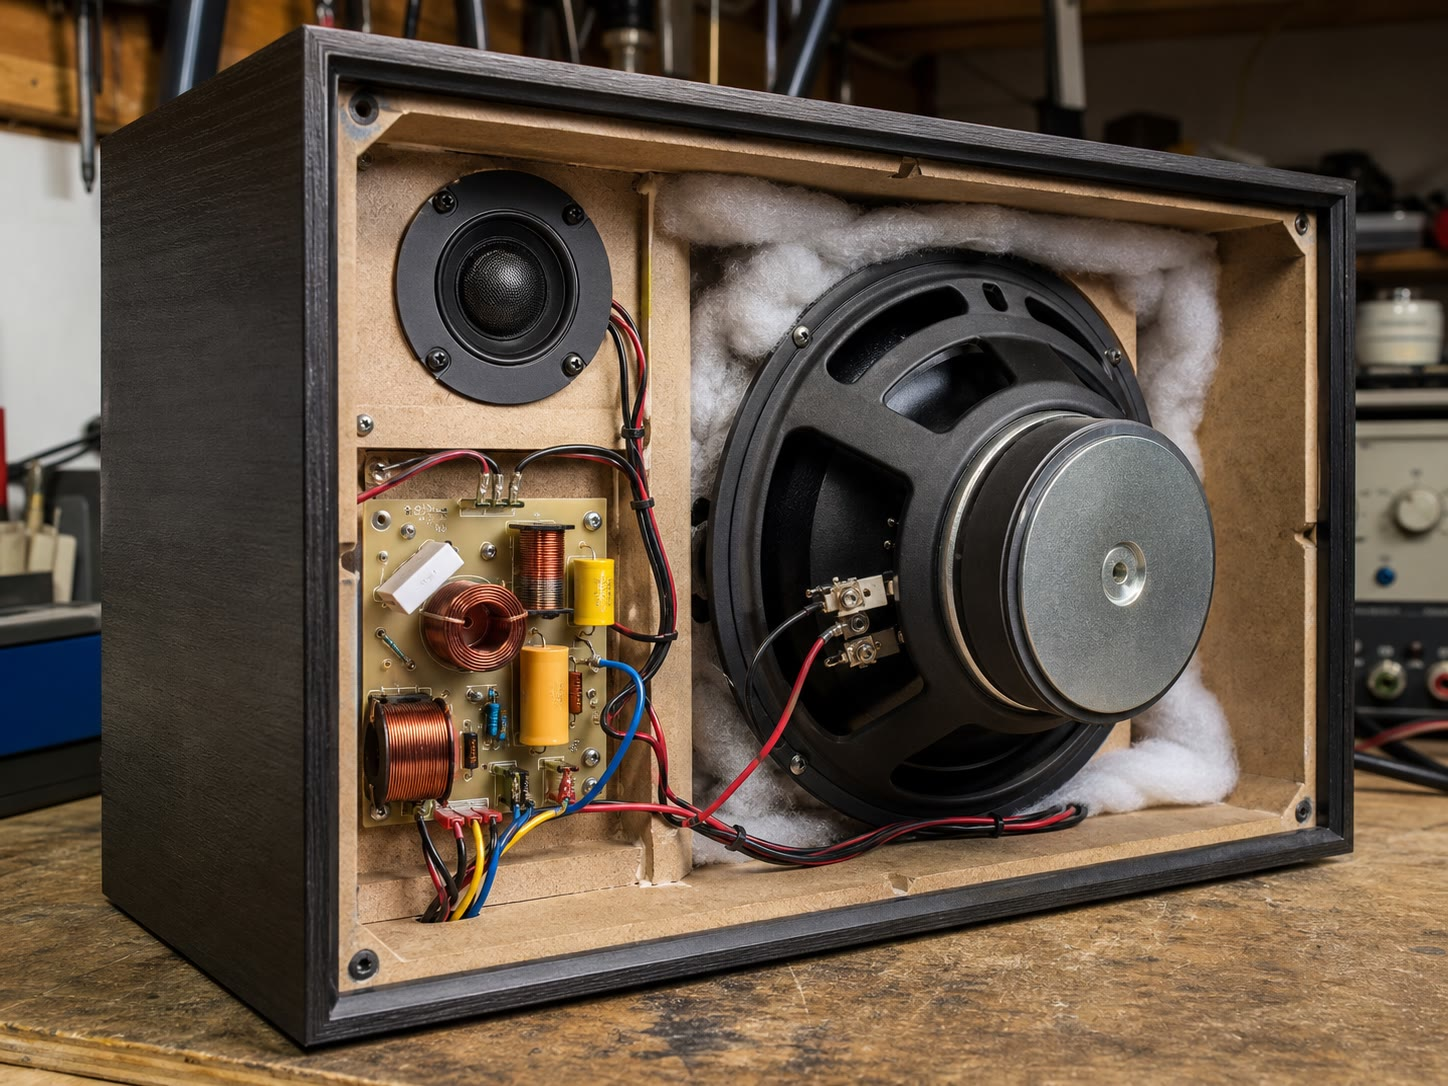
\includegraphics[width=0.50\linewidth]{images/book3/ai/b3-09-loudspeaker-crossover.jpg}

{\small 二分频扬声器内部：分频器的线圈与电容器构成低通与\omterm{prop:b1:filters-transfer-functions:highpass1}{高通滤波器}，分别将低音送往低音单元，将高音送往高音单元。}
\end{omfigure}

\section{问题：扬声器分频器}

\begin{problem}[{周末问题——低音单元、高音单元、线圈与电容器：无源分频器如何分配音乐，
为何最简单的一种会把低音漏入高音单元，
以及真实的音圈会对
设计产生何种影响}]
\label{pb:b1:filters-transfer-functions:1}
低音单元与高音单元首先被建模为纯电阻
$R = \qty{8.0}{\ohm}$。放大器是一个理想\omterm{def:b1:dc-circuits:sources}{电压源}
$\underline U_e$。分频频率为 $f_c = \qty{2.0}{kHz}$。

\medskip
\noindent\textbf{第一部分——一阶分频器。}
低音单元经串联线圈 $L$ 供电，高音单元经
串联电容器 $C$ 供电。
\begin{enumerate}
  \item 定义各支路的\omterm{def:b1:filters-transfer-functions:H}{传递函数}（驱动器两端的
        \omterm{def:b1:dc-circuits:voltage}{电压}与 $\underline U_e$ 之比），并给出\omterm{def:b1:filters-transfer-functions:bode}{分贝}\omterm{def:b1:filters-transfer-functions:H}{增益}。
  \item 证明低音支路为一阶低通\omterm{def:b1:filters-transfer-functions:H}{滤波器}，
        并求其\omterm{def:b1:filters-transfer-functions:bode}{截止频率} $\omega_c$（用 $R$ 与 $L$ 表示）。
  \item 计算 $L$，取 $f_c = \qty{2.0}{kHz}$。
  \item 证明高音支路为一阶\omterm{prop:b1:filters-transfer-functions:highpass1}{高通滤波器}，
        给出 $\omega_c$，并计算 $C$。
  \item 给出各驱动器在 $f_c$、\qty{200}{Hz}
        及 \qty{20}{kHz} 处的\omterm{def:b1:filters-transfer-functions:bode}{分贝}\omterm{def:b1:filters-transfer-functions:H}{增益}。
  \item 证明对任意频率均有 $G_L^2 + G_H^2 = 1$。这对放大器所提供的功率
        意味着什么？
  \item 给出 $f_c$ 处各支路的\omterm{def:b1:wave-propagation:signal}{相位}，
        并求两驱动器\omterm{def:b1:dc-circuits:voltage}{电压}在该处的\omterm{def:b1:wave-propagation:signal}{相位}差。
  \item 两条响应曲线的斜率为多少（以 dB/倍频程计，
        远离 $f_c$ 时）？
\end{enumerate}

\medskip
\noindent\textbf{第二部分——二阶分频。}
低音驱动器现在经一个串联线圈 $L$ 馈电，
且有一电容器 $C$ 与驱动器并联。
\begin{enumerate}[resume]
  \item 证明 $\underline H = 1/(1 - LC\omega^2 + jL\omega/R)$。
  \item 求 $\omega_0$ 与 $Q$，并用 $L$、$C$、$R$ 表示。
  \item 当 $Q = 1/\sqrt2$ 时，证明 $G = 1/\sqrt{1 + (\omega/\omega_0)^4}$，
        并证明在 $\omega_0$ 处\omterm{def:b1:filters-transfer-functions:H}{增益}为 \qty{-3}{dB}。
  \item 求 $L$ 与 $C$，使 $f_0 = \qty{2.0}{kHz}$ 且 $Q = 1/\sqrt2$。
  \item 计算在 \qty{4}{kHz} 与 \qty{8}{kHz} 处的\omterm{def:b1:filters-transfer-functions:bode}{分贝}\omterm{def:b1:filters-transfer-functions:H}{增益}，
        并由此求出斜率（以 dB/倍频程计）。
  \item 高音支路互换 $L$ 与 $C$ 的角色（串联 $C$，
        并联 $L$），
        直接写出其\omterm{def:b1:filters-transfer-functions:H}{传递函数}。
  \item 求各支路在 $f_0$ 处的\omterm{def:b1:wave-propagation:signal}{相位}。高音单元
        的接线应作何改动，为什么？
\end{enumerate}

\medskip
\noindent\textbf{第三部分——音乐经过分频网络。}
\begin{enumerate}[resume]
  \item 一个 \qty{220}{Hz} 的大提琴音含有直至第 20 次的谐音。
        在一阶分频网络下，哪些谐音主要流向
        高音单元？
  \item 第 9 次谐音会怎样？
  \item 以 \qty{1.0}{kHz} 的方波作测试\omterm{def:b1:wave-propagation:signal}{信号}。在一阶分频下，
        求各支路对其基波、
        三次和五次谐波的\omterm{def:b1:filters-transfer-functions:H}{增益}。
  \item 放大器意外产生 \qty{1}{V} 直流偏移，哪一个驱动器
        受到保护，它又是由什么保护的？
  \item 在一阶分频下，\qty{500}{Hz} 音调到达高音单元的\omterm{def:b1:dc-circuits:voltage}{电压}
        和功率各占多大比例？
        二阶分频时又如何？
        这对高音单元的安全为何重要？
\end{enumerate}

\medskip
\noindent\textbf{第四部分——真实的音圈。}
低音驱动器实际上相当于 $R = \qty{8.0}{\ohm}$ 与音圈
电感 $L_{vc} = \qty{0.50}{mH}$ 串联。
\begin{enumerate}[resume]
  \item 求低音驱动器在 \qty{2}{kHz} 和
        \qty{8}{kHz} 处的\omterm{def:b1:sinusoidal-impedance:impedance}{阻抗}模。
  \item 用此\omterm{def:b1:sinusoidal-impedance:impedance}{阻抗}重新计算一阶低音\omterm{def:b1:filters-transfer-functions:H}{增益}在 \qty{2}{kHz} 和
        \qty{8}{kHz} 处的值，并与理想情形的
        \qty{-3}{dB} 和 \qty{-12.3}{dB} 相比较。滚降发生了什么变化？
  \item 一个“佐贝尔网络”——由 $R_z = R$ 与 $C_z =
        L_{vc}/R^2$ 串联构成——与低音驱动器并联。证明
        该组合在所有频率下都表现为纯电阻 $R$，
        并求 $C_z$。
  \item 放大器向 \qty{8}{\ohm} 负载输出 \qty{50}{W} 功率，
        其\omterm{def:b1:dc-circuits:voltage}{电压}\omterm{def:b1:sinusoidal-impedance:rms}{有效值}为多少，各驱动器在 $f_c$（一阶分频）处
        接收的功率为多少？在 \qty{500}{Hz} 时，
        有多少到达高音单元？
  \item 总结各种权衡：斜率、\omterm{def:b1:wave-propagation:signal}{相位}、元件数量、
        高音单元的保护，以及是否需要佐贝尔网络。
\end{enumerate}
\end{problem}
